\chapter{Παραγωγή Codebooks}
\label{chapter:chap4}

\section{Εισαγωγή}
\label{section:sect41}

\indent Σε αυτό το κεφάλαιο θα παρουσιαστεί ο τρόπος με τον οποίο εκπαιδεύτηκε ο kmeans (training) και με ποία δεδομένα (training set). Επίσης θα δειχθεί ο τρόπος εξαγωγείς των δεδομένων από τον H.264.

\section{Επιλογή του training set}
\label{section:sect42}

\indent Όπως εξηγήθηκε στο Κεφάλαιο~\ref{chapter:chap2} τα δεδομένα που ένας κωδικοποιητής συμπιέζει είναι τα residuals και όχι τα pixels. Πρέπει να είναι ξεκάθαρο πως τα residuals μαζί με τα motion vector μας δίνουν όλη την πληροφορία για να ανακατασκευάσουμε ένα καρέ. Αν δεν έχει παρεμβληθεί η κβαντοποίηση τότε το ανακατασκευασμένο με το αυθεντικό καρέ θα είναι πανομοιότυπα. Έτσι λοιπόν επιλέχθηκαν τα residuals να είναι το training set του kmeans.

\indent Μέχρι τώρα έχει γίνει σαφές πως για κάθε καρέ διάστασης W*H pixels υπάρχουν W*H residuals. Επομένως είναι εφικτό να τεμαχίσουμε το καρέ σε d*d blocks οπού d η διάσταση του training set. Το d έχει τον μοναδικό περιορισμό ότι πρέπει να είναι μικρότερο από την διάσταση του block του encoder, στον H.264 που αυτή η διπλωματική βασίστηκε $blocksize\in[2*2,16*16]$ και μπορεί να ρυθμιστεί ανάλογα. Η διάσταση που επιλέχθηκε είναι το $d=4$ που πληρεί το κριτήριο "blocksize" και είναι η προεπιλεγμένη τιμή blocksize στον H.264. Έστω ένα καρέ ανάλυσης 720*480 με YUV420 τότε συνολικά έχουμε $720*480*1.5=518400$ pixels και $ \frac{518400}{4*4} = 32400 $ training vectors.

\indent Τα βίντεο που θα μας έδινα το training set έπρεπε να επιλεχθούν προσεκτικά γιατί χρειάζεται να πληρούν κάποιες προϋποθέσεις.
\begin{itemize}
    \item Θα πρέπει να υπάρχει ένας ικανοποιητικός αριθμός από καρέ για να μπορέσουμε να έχουμε αντιπροσωπευτικά στατιστικά. Στην διπλωματική χρησιμοποιήθηκαν 2600 καρέ από 10 διαφορετικά βίντεο ανάλυσης 720*480. Αρά συνολικά είχαμε 84240000 training vectors που θεωρείται ικανοποιητικός αριθμός.
    \item Το περιεχόμενο των βίντεο παίζει καθοριστικό ρόλο για το PSNR του VQ όταν δοκιμάζετε σε βίντεο εκτός του training set. Για παράδειγμα εάν το training set μας δε περιλαμβάνει σκηνές που απεικονίζουν βουνά τότε αν κωδικοποιηθεί ένα βίντεο που περιέχει σκηνές από βουνά θα έχουμε χαμηλά PSNR (φαινόμενο mismatch). Τα 10 βίντεο που χρησιμοποιήθηκαν είχαν διαφορετικές σκηνές και μπορούμε να δούμε κάποια στιγμιότυπα στο Σχήμα~\ref{fig:trainingset}.
\end{itemize}

\indent Θεωρητικά το καλύτερο training set θα ήταν όλα τα βίντεο που κυκλοφορούν στον πλανήτη (talk shows, ταινίες, αθλήματα κ.τ.λ) αλλά τότε η πολυπλοκότητα του προβλήματος αυξάνεται σε επίπεδα που οι σημερινοί υπολογιστές δεν μπορούν να λύσουν σε εύλογο χρονικό διάστημα.
        
\begin{table}[p]
\centering
\begin{tabular}{c c}
    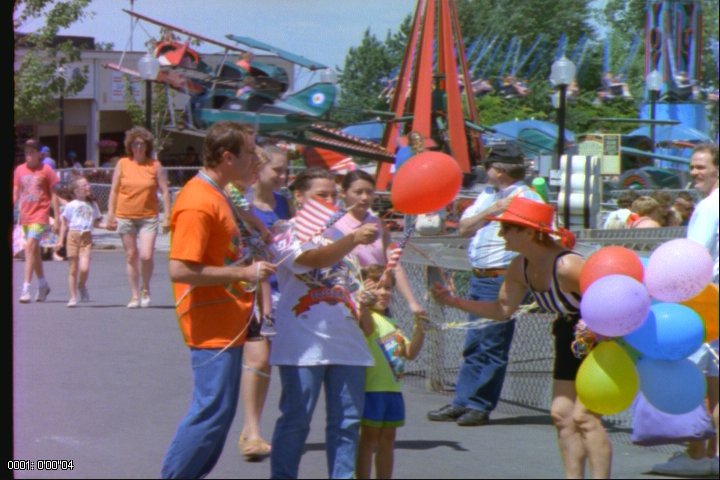
\includegraphics[height=4.0cm]{chapter4/frames/src13.png}
    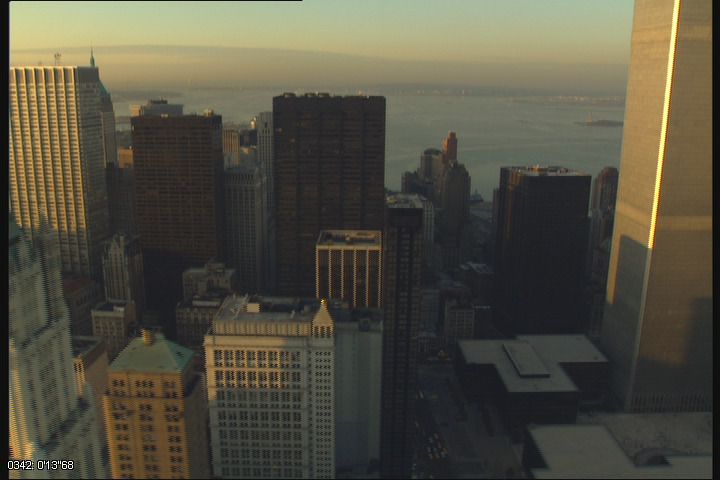
\includegraphics[height=4.0cm]{chapter4/frames/src14.png}\\
    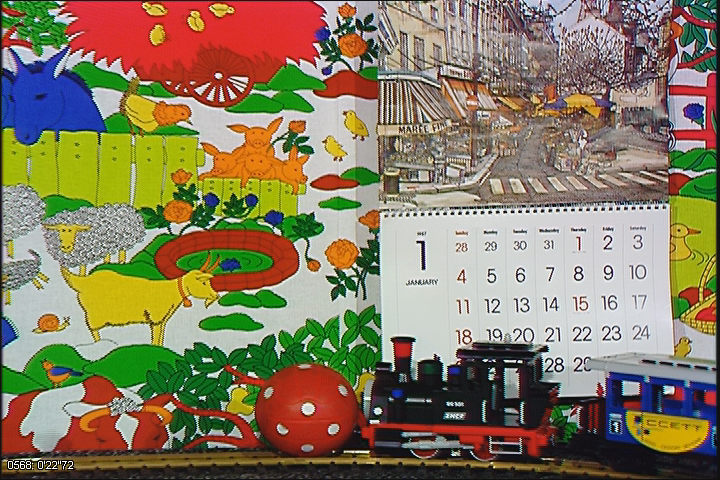
\includegraphics[height=4.0cm]{chapter4/frames/src15.png}
    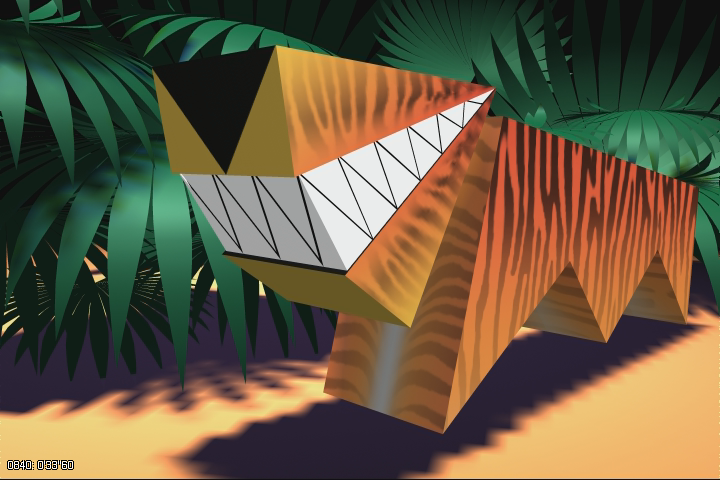
\includegraphics[height=4.0cm]{chapter4/frames/src16.png}\\
    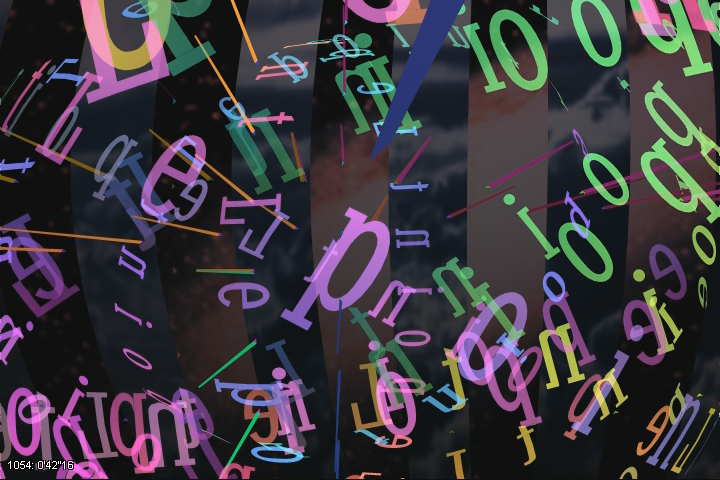
\includegraphics[height=4.0cm]{chapter4/frames/src17.png}
    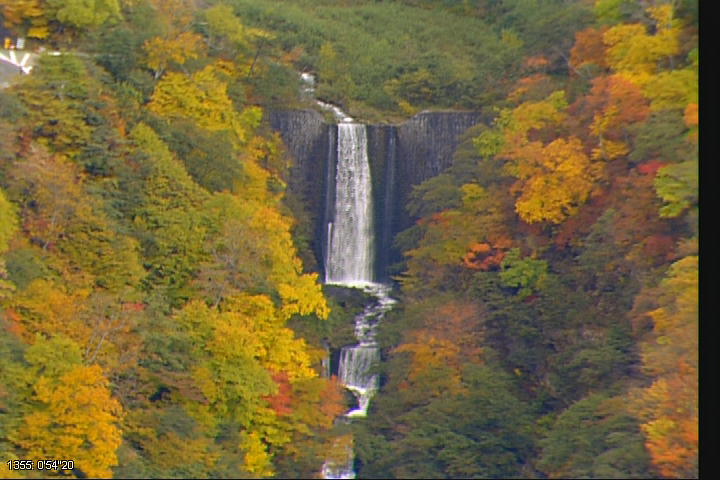
\includegraphics[height=4.0cm]{chapter4/frames/src18.png}\\
    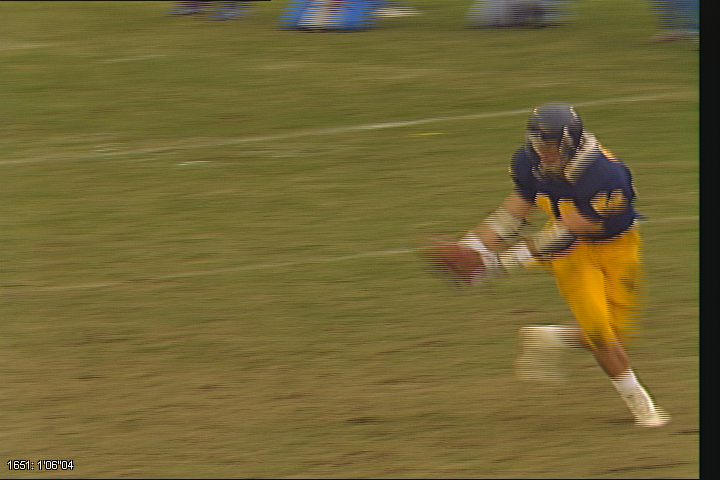
\includegraphics[height=4.0cm]{chapter4/frames/src19.png}
    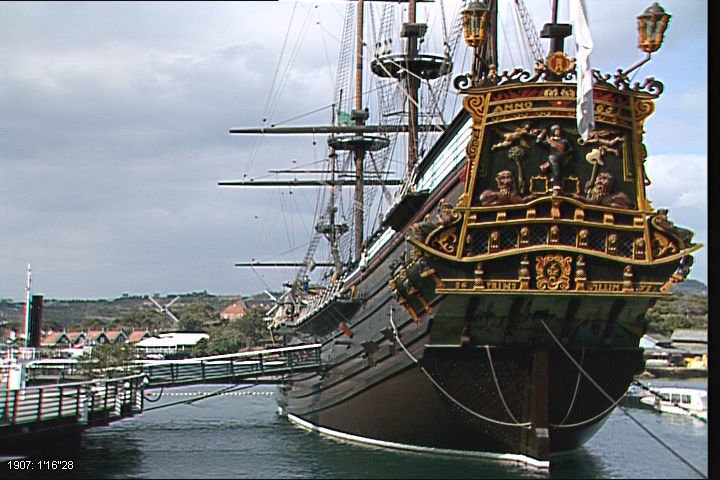
\includegraphics[height=4.0cm]{chapter4/frames/src20.png}\\
    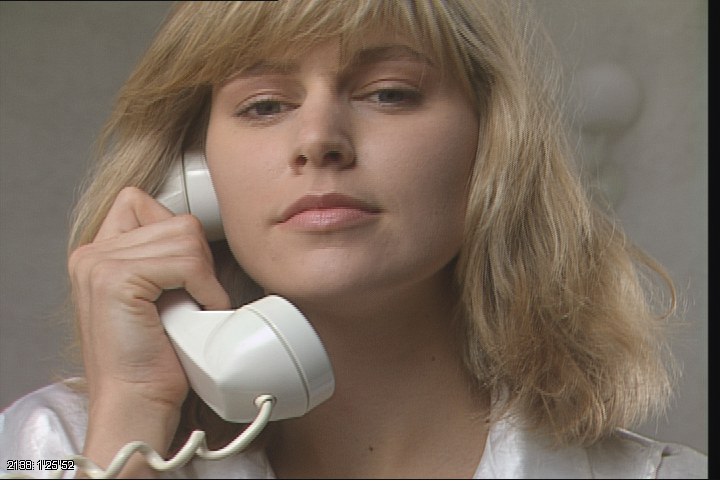
\includegraphics[height=4.0cm]{chapter4/frames/src21.png}
    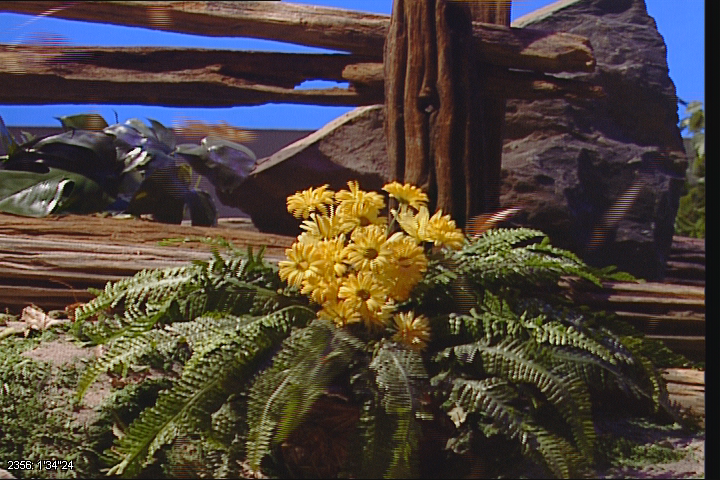
\includegraphics[height=4.0cm]{chapter4/frames/src22.png}
\end{tabular}
\caption{Training βίντεο.}
\label{fig:trainingset}
\end{table}

\section{Εξαγωγή training set από τον H.264}
\label{section:sect43}

\indent 